In this section we will be demonstrating the experimental evaluation of the Sentiment Analysis algorithm we have implemented; which is a crucial part of our framework, and we will have a look on at the execution time of the whole framework. In addition to this we will be showing the results that we obtain while collecting the data; the considered data collection period was: \emph{April 1st, 2014 - April 30th, 2014}. We have to have in mind that we will be considering only working days from \emph{Monday - Friday}; and if it was some holiday in this period, it was not considered in the analysis because the \gls{NYSE} is close in this period.

\section{Experimental evaluation.}

In this section we will be showing the behavior of the framework in it's most important and CPU time consuming part: \emph{The Polarity Analysis}; as shown in the section \ref{sentimentAnalysis}. In addition to the experimental evaluation, we have implemented \emph{multi-threading} in our framework, and we will be demonstrating experimentally how it \emph{speedup} the framework.

We will be using the \emph{Linear least squares} to get experimentally the complexity of the algorithm. \emph{Linear least squares \cite{L2014} is an approach fitting a mathematical or statistical model to data in cases where the idealized value provided by the model for any data point is expressed linearly in terms of the unknown parameters of the model. The resulting fitted model can be used to summarize the data, to predict unobserved values from the same system, and to understand the mechanisms that may underlie the system.}

We are presenting the results of this particular section in the table \ref{tab:wordsTime} and graphically in the figure \ref{fig:wordsTime} and even if the \emph{Linear least squares} (figure \ref{fig:Experiment_001}) method suggest a degree four complexity according to the data, we will take the complexity in degree 3, because of the amount of nested loops in the code (3). The equation that fits the better has the following form: 
\[4.98946x10^-7 x^3-0.00239705 x^2+4.28487 x-422.422\] 
which asymptotically is equivalent on average to 
\[\theta(n^3)\] 
We can verify the details of the \emph{Linear least squares} method in the following link:
\\\\
\url{http://www.wolframalpha.com/input/?i=fit+%2814%2C+229.7524129%29%2C%281014%2C+803.3164669%29%2C%282014%2C+1601.227397%29%2C%283014%2C+2921.279661%29%2C%284014%2C+3171.105263%29%2C%285014%2C+5282.681818%29%2C%286014%2C+3400.888889%29%2C%287014%2C+9654.75%29%2C%288014%2C+11768.33333%29%2C%289014+%2C+4507.2%29}

\begin{figure}\centering
	\caption{Number of words vs. Execution time (ms)}\label{fig:wordsTime}
	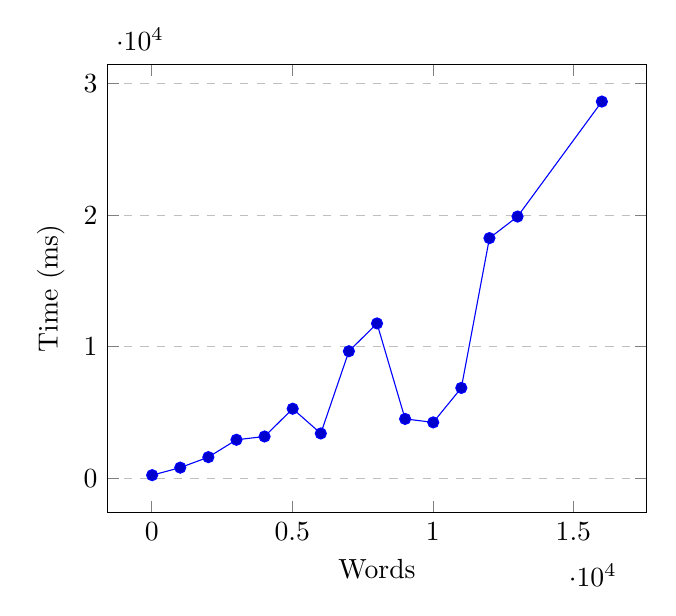
\begin{tikzpicture}
		\begin{axis}[ 
			xlabel=Words,
			ylabel=Time (ms),
			ymajorgrids=true,
			grid style=dashed,
  				]	 
			\addplot coordinates {
				(14, 229.7524129)
				(1014, 803.3164669)
				(2014, 1601.227397)
				(3014, 2921.279661)
				(4014, 3171.105263)
				(5014, 5282.681818)
				(6014, 3400.888889)
				(7014, 9654.75)
				(8014, 11768.33333)
				(9014 , 4507.2)
				(10014, 4242.875)
				(11014, 6866)
				(12014, 18255)
				(13014, 19895)
				(16014, 28639.5)
				};
		\end{axis}
	\end{tikzpicture}
\end{figure}

\begin{table}\centering
	\caption{Number of words vs. Execution time (ms)}\label{tab:wordsTime}
   	\begin{tabular}{ | p{4cm\textwidth} | p{4cm\textwidth} |}
   	\hline

\textbf{Number of Words}  & \textbf{Average Execution time (ms)}       \\\hline
14-1013     & 229.7524129 \\\hline
1014-2013   & 803.3164669 \\\hline
2014-3013   & 1601.227397 \\\hline
3014-4013   & 2921.279661 \\\hline
4014-5013   & 3171.105263 \\\hline
5014-6013   & 5282.681818 \\\hline
6014-7013   & 3400.888889 \\\hline
7014-8013   & 9654.75     \\\hline
8014-9013   & 11768.33333 \\\hline
9014-10013  & 4507.2      \\\hline
10014-11013 & 4242.875    \\\hline
11014-12013 & 6866        \\\hline
12014-13013 & 18255       \\\hline
13014-14013 & 19895       \\\hline
16014-17013 & 28639.5    \\\hline

    \end{tabular}
\end{table}

\begin{figure}\centering
	\includegraphics[scale=0.65]{Experiment_001}
	\caption{Least-squares Analysis - Words}\label{fig:Experiment_001}
\end{figure}


We are presenting the results of this particular section in the table \ref{tab:patternTime} and graphically in the figure \ref{fig:patternTime}. In the case of the patterns, this is strongly related to the complexity of the algorithm, because number of patterns will define how many loops will be executing; again, we perform the \emph{Linear least squares} method, in order to figure out the average time complexity of the algorithm. We will accept the linear equation, and it look as follows:
\[23.3226 x-2619.46\] 
which asymptotically is equivalent on average to 
\[\theta(n)\] 
We can verify the details of the \emph{Linear least squares} method in the following link:	
\\\\	
\url{http://www.wolframalpha.com/input/?i=fit+%2899+%2C+286.5746529+%29%2C%28199%2C+1430.8487+%29%2C%28299%2C+3201.441441+%29%2C%28399%2C+5272.302326+%29%2C%28499%2C+6610.857143+%29%2C%28599%2C+15193.8+%29%2C%28699%2C+21042.5+%29%2C%28799%2C+11245+%29%2C%28899%2C+15079+%29%2C%28999%2C+25786.33333+%29%2C%281099%2C+19710%29}

\begin{figure}\centering
	\caption{Number of patterns vs. Average execution time (ms)}\label{fig:patternTime}
	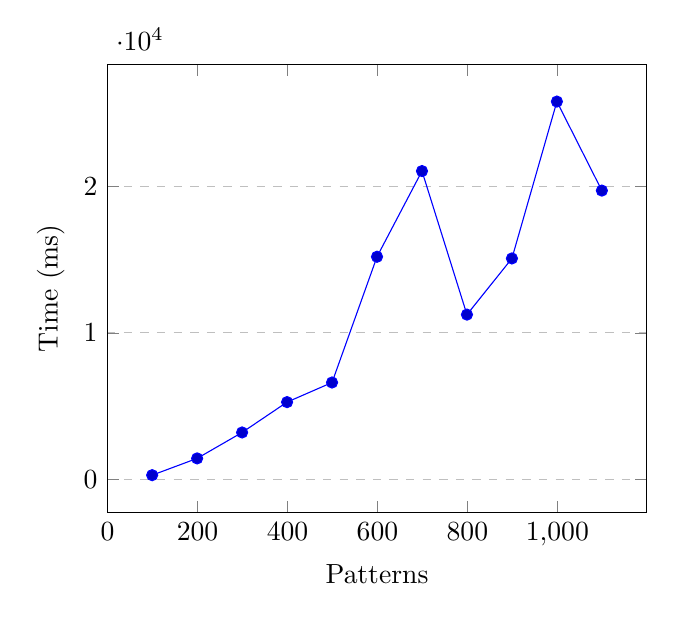
\begin{tikzpicture}
		\begin{axis}[ 
			xlabel=Patterns,
			ylabel=Time (ms),
			ymajorgrids=true,
			grid style=dashed,
  				]	 
			\addplot coordinates {
(99       , 286.5746529 )
(199    , 1430.8487   )
(299    , 3201.441441 )
(399    , 5272.302326 )
(499    , 6610.857143 )
(599    , 15193.8     )
(699    , 21042.5     )
(799    , 11245       )
(899    , 15079       )
(999    , 25786.33333 )
(1099  , 19710      )
				};
		\end{axis}
	\end{tikzpicture}
\end{figure}


\begin{table}\centering
	\caption{Number of patterns vs. Average execution time (ms)}\label{tab:patternTime}
   	\begin{tabular}{ | p{4cm\textwidth} | p{4cm\textwidth} |}
   	\hline
\textbf{Number of Patterns}  & \textbf{Average Execution time}       \\\hline
0-99       & 286.5746529 \\\hline
100-199    & 1430.8487   \\\hline
200-299    & 3201.441441 \\\hline
300-399    & 5272.302326 \\\hline
400-499    & 6610.857143 \\\hline
500-599    & 15193.8     \\\hline
600-699    & 21042.5     \\\hline
700-799    & 11245       \\\hline
800-899    & 15079       \\\hline
900-999    & 25786.33333 \\\hline
1000-1099  & 19710      \\\hline

    \end{tabular}
\end{table}

\begin{figure}\centering
	\includegraphics[scale=0.65]{Experiment_002}
	\caption{Least-squares Analysis - Patterns}\label{fig:Experiment_002}
\end{figure}


\subsection{Multi-Threading Performance}

We are presenting the results of this particular section in the table \ref{tab:threadsTime} and graphically in the figures: \ref{fig:threadsTime}. For this part we will cite professor Tvrdík \cite[p. 3-9]{T2011} in the chapter \emph{Performance and Scalability of parallel algorithms.}, where there are some metrics in order to measure the performance of parallel algorithms. We will describe several of this metrics in order to analyze the parallelism of our framework.

\begin{itemize}
	\item \emph{Parallel time T(n,p)}: Is the time elapsed from the beginning of a p-processor (In our case we will consider software threads) parallel algorithm solving a problem instance of size \emph{n} until the last processor finishes the execution. \emph{T(n,p)} is obtained by \emph{counting} or by \emph{measuring the total time complexity} of:
	\begin{itemize}
		\item \emph{parallel computationl} steps. e.g., arithmetic operations.
		\item \emph{parallel communication} steps. i.e., transfers and exchanges of data between processors.
	\end{itemize}	
	Due to the second component \emph{T(n,p)} depends on the architecture of a parallel computer. Therefore the performance evaluation of a parallel algorithm must \emph{always} consider the architecture. In a specific algorithm, \emph{p} is always chosen as a suitable function of \emph{n}.

	\item \emph{Parallel Speedup S(n,p)}: If both, sequential and parallel algorithm with \emph{p} processors are executed under the same conditions, the best speedup we can hope is for \emph{p}. Due to the communication overhead, such a speedup is achievable only if the solution of the problem contains enough parallelism, the communication part is negligible, and all the processors perform only useful computation under ideal load balancing and synchronization. In practice, a linear speedup \emph{kp} for some constant 0 < k <1 is quite satisfactory.
	
	\item \emph{Parallel cost C(n,p)}: 
	\[C(n,p) = p * T(n,p) \] 
	This metric is a bit coarse-grained. It is actually an upper estimate of the operational complexity. It gives the total number of operations as if all processors were active since the beginning till the end (like the slowest processor). But this is what parallel systems with job schedulers typically allow: prior to a parallel computation, a user job is assigned p processors and these are released only after the whole parallel computation has finished. In such systems, \emph{C(n,p)} is a useful metric, since idling processors or processors that finished their subtasks faster are useless for the other users until the whole computation finishes. Since any parallel algorithm can be trivially simulated on a uniprocessor machine with multiprogramming, we get that \emph{The parallel Cost, cannot be less than the complexity of the best sequential algorithm:}
	\[C(n,p) = \Omega(SU(n)) \] 
	\emph{In the best case, the cost is of the same order as the sequential complexity:}
	\[C(n,p) = O(SU(n)) \] 
	
	\item \emph{Parallel Efficiency E(n,p)}
	\[E(n,p) = \frac{SU(n)}{C(n,p)} = \frac{S(n,p) * T(n,p)}{p * T(n,p)} =  \frac{S(n,p)}{p} \leq 1 \] 
	Basically, the Parallel efficiency is the speedup per processor.
\end{itemize}

Now, that we prepare a theoretical background, we will be mentioning the characteristics of the hardware where the tests have been performed, and after this we will be introducing the experimental results, which are shown in the table \ref{tab:threadsTime}.

\begin{itemize}
	\item CPU: 1.86 GHz Intel Core 2 Duo
	\item Memory:  4 GB, 1067 MHz DDR3
	\item Operative System: OS X 10.8.5 (12F45)
	\item Hard drive: APPLE SSD TS128C Media
	\item Considered size of the problem: \emph{n=35}
\end{itemize}

\begin{table}\centering
	\caption{Multi-Threading Performance Analysis}\label{tab:threadsTime}
   	\begin{tabular}{ | p{2.5cm\textwidth} | p{2.5cm\textwidth} | p{2.5cm\textwidth} | p{2.5cm\textwidth} | p{2.5cm\textwidth} |}
   	\hline
\textbf{Number of threads} & \textbf{Execution time (s) T(n,p)}& \textbf{Speedup S(n,p)} & \textbf{Efficiency E(n,p)} & \textbf{Cost C(n,p)} \\\hline
1               & 223.816 	&	 1			&	1			&	223.816          \\\hline
2               & 124.441	&	 1.79857121	&	0.899285605	&	248.882           \\\hline
3               & 103.705	&	 2.158198737 	&	0.719399579	&	311.115           \\\hline
4               & 111.66	&	 2.004442056	&	0.501110514	&	446.64            \\\hline
5               & 101.099	&	 2.213830008	&	0.442766002	&	505.495           \\\hline
6               & 100.934	&	 2.217449026	&	0.369574838	&	605.604           \\\hline
7               & 95.115	&	 2.353109394 	&	0.336158485	&	665.805            \\\hline
8               & 89.632	&	 2.497054623	&	0.312131828	&	717.056            \\\hline
9               & 91.493	&	 2.446263649	&	0.271807072	&	823.437            \\\hline
10              & 93.347	&	 2.397677483	&	0.239767748	&	933.47            \\\hline
11              & 124.689	&	 1.794993945	&	0.163181268	&	1371.579           \\\hline
12              & 131.235	&	 1.705459672	&	0.142121639	&	1574.82           \\\hline
13              & 134.524	&	 1.6637626	&	0.127981738	&    1748.812      \\\hline

    \end{tabular}
\end{table}

Now that we have the execution data, we will visualize each of them in a plot. \emph{Time complexity T(n,p)} can be visualized in the figure \ref{fig:threadsTime}, \emph{Cost C(n,p)} in the figure \ref{fig:threadsCost}, \emph{Speedup S(n,p)} in the figure \ref{fig:threadsSpeedup}, and the \emph{Efficiency E(n,p)} in the figure {fig:threadsEfficiency}.

\begin{figure}\centering
	\caption{Number of threads vs Average execution time (s)}\label{fig:threadsTime}
	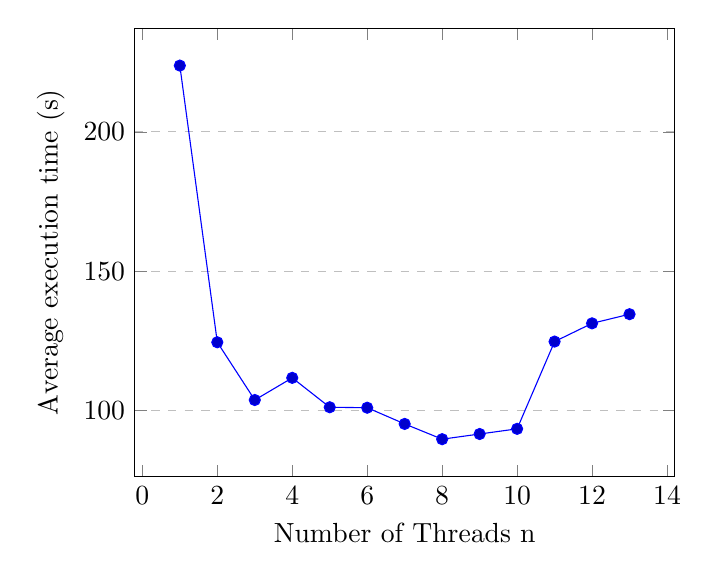
\begin{tikzpicture}
		\begin{axis}[ 
			xlabel=Number of Threads n,
			ylabel=Average execution time (s),
			ymajorgrids=true,
			grid style=dashed,
  				]	 
			\addplot coordinates {
(1               , 223.816           )
(2               , 124.441           )
(3               , 103.705           )
(4               , 111.66            )
(5               , 101.099           )
(6               , 100.934           )
(7               , 95.115            )
(8               , 89.632            )
(9               , 91.493            )
(10              , 93.347            )
(11              , 124.689           )
(12              , 131.235           )
(13              , 134.524          )
				};
		\end{axis}
	\end{tikzpicture}
\end{figure}

\begin{figure}\centering
	\caption{Number of threads vs Cost}\label{fig:threadsCost}
	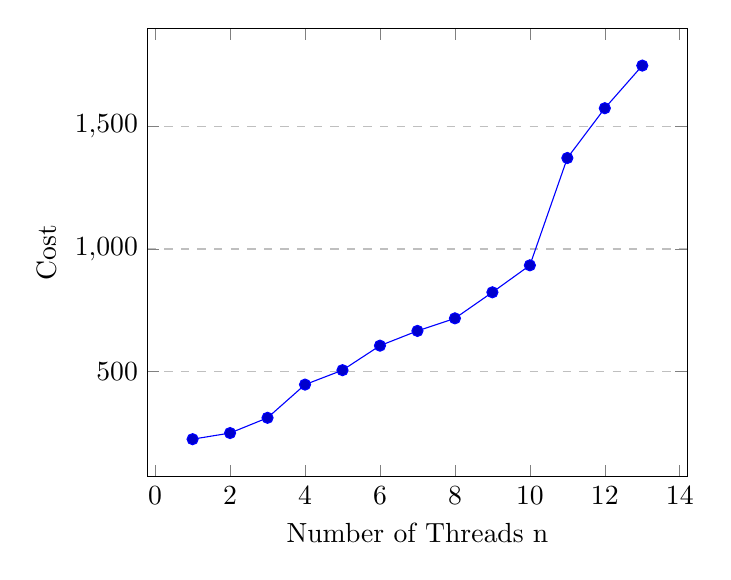
\begin{tikzpicture}
		\begin{axis}[ 
			xlabel=Number of Threads n,
			ylabel=Cost,
			ymajorgrids=true,
			grid style=dashed,
  				]	 
			\addplot coordinates {
(1               , 223.816            )
(2               , 248.882            )
(3               , 311.115           )
(4               , 446.64            )
(5               , 505.495          )
(6               , 605.604           )
(7               , 665.805            )
(8               , 717.056            )
(9               , 823.437          )
(10              , 933.47            )
(11              , 1371.579           )
(12              , 1574.82         )
(13              , 1748.812          )
				};
		\end{axis}
	\end{tikzpicture}
\end{figure}

\begin{figure}\centering
	\caption{Number of threads vs Speed up}\label{fig:threadsSpeedup}
	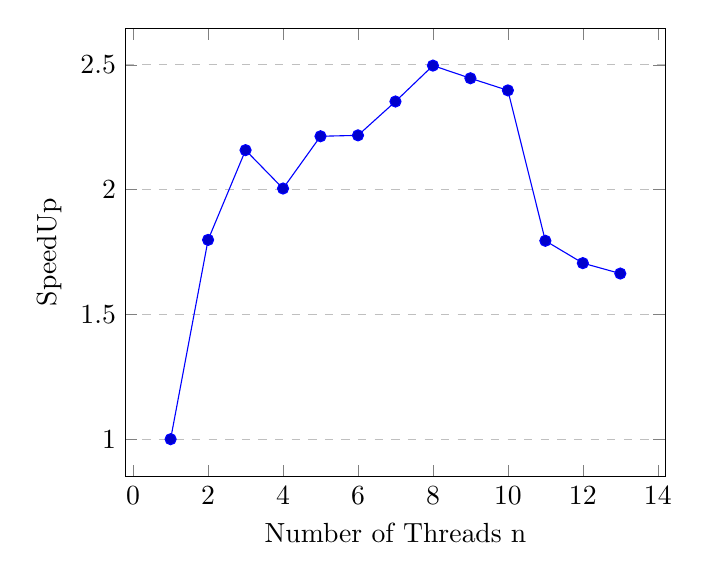
\begin{tikzpicture}
		\begin{axis}[ 
			xlabel=Number of Threads n,
			ylabel=SpeedUp,
			ymajorgrids=true,
			grid style=dashed,
  				]	 
			\addplot coordinates {
(1               , 1           )
(2               , 1.79857121  )
(3               , 2.158198737 )
(4               , 2.004442056 )
(5               , 2.213830008 )
(6               , 2.217449026 )
(7               , 2.353109394 )
(8               , 2.497054623 )
(9               , 2.446263649 )
(10              , 2.397677483 )
(11              , 1.794993945 )
(12              , 1.705459672 )
(13              , 1.6637626   )
				};
		\end{axis}
	\end{tikzpicture}
\end{figure}

\begin{figure}\centering
	\caption{Number of threads vs Efficiency}\label{fig:threadsEfficiency}
	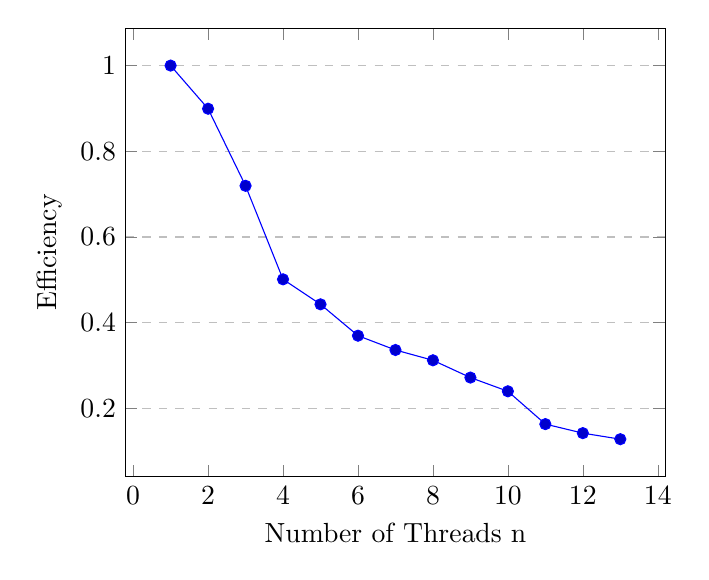
\begin{tikzpicture}
		\begin{axis}[ 
			xlabel=Number of Threads n,
			ylabel=Efficiency,
			ymajorgrids=true,
			grid style=dashed,
  				]	 
			\addplot coordinates {
(1               , 1           )
(2               , 0.899285605  )
(3               , 0.719399579 )
(4               , 0.501110514 )
(5               , 0.442766002 )
(6               , 0.369574838 )
(7               , 0.336158485 )
(8               , 0.312131828 )
(9               , 0.271807072 )
(10              , 0.239767748 )
(11              , 0.163181268  )
(12              , 0.142121639 )
(13              , 0.127981738 )
				};
		\end{axis}
	\end{tikzpicture}
\end{figure}


Now that we presented the collected data, we would like to estimate an approximate time complexity that would fit our \emph{Time Complexity T(n,p)} data. For that we will apply the method described before: \emph{Linear least squares}. After the analysis, we will adopt for our data the following equation for the \emph{Time Complexity T(n,p)}.
\[191.451-54.8072 log(x)\] 
which asymptotically is equivalent on average to 
\[\theta(log(x))\] 
We can verify the details of the \emph{Linear least squares} method in the figure \ref{fig:Experiment_003} or in the following link:	
\\\\
\url{http://www.wolframalpha.com/input/?i=fit+%281+%2C+223.816%29%2C%282+%2C+124.441%29%2C%283+%2C+103.705%29%2C%284+%2C+111.66+%29%2C%285+%2C+101.099%29%2C%286+%2C+100.934%29%2C%287+%2C+95.115+%29%2C%288+%2C+89.632+%29}
\\\\

\begin{figure}\centering
	\includegraphics[scale=0.65]{Experiment_003}
	\caption{Least-squares Analysis - Threads}\label{fig:Experiment_003}
\end{figure}

In order to explain our results we will cite one article \cite{SF2008}, Our first problem was to determine the optimal number of threads that would be suitable for our task. What we did was to run the framework with several number of threads (from 1 to 13) in our limited hardware environment, and according to the average of the results of the execution time versus the number of threads (as shown in table \ref{tab:threadsTime} and figure \ref{fig:threadsTime}) and the theory; there is some \emph{threshold} \cite[p. 9]{T2011} where when p increases, the time decreases, but after this \emph{threshold}, the decreasing time is slower and slower with increasing \emph{p}; which means that the efficiency decreases and the cost starts to grow. Each Parallel Algorithm has its own flexibility to choose \emph{n} if \emph{p} changes or to choose \emph{p} if \emph{n} changes. After this, comes the concept of \emph{Time Scallability} (shown on the figure \ref{fig:threadsTime}), which is the minimum p, such that time is asymptotically optimal. If we analyze the figure \ref{fig:threadsTime} or the table \ref{tab:threadsTime} we can observe that after some \emph{threshold}, after adding more and more \emph{threads}, the time became worser; so after this, we will choose the number of threads that will keep a good performance without degrading the Execution time; which in our case will be 8 threads. 

Earlier we mention that we would explain the "why" of our results with such a limited hardware environment (2 cores). An approach of this answer was given in the section \ref{concurrency}; which states that the sequential version of our framework makes the processor \emph{iddle} for a long time (Almost "light years" in processor time :-)), and all this time the processor is waiting for download or I/O operations to finish. And after implementing 8 threads, our \emph{Time T(n,p)} and \emph{Speedup S(n,p)} are maximum in our environment. 

We can conclude that this improvement make an important impact on the performance of the framework \emph{for "free"}; because we are using exactly the same hardware. And the same behavior is expected for bigger \emph{sizes of the problem "n"} in larger \emph{infrastructures}.

\section{Results.}

In order to present the results, we will present the analyzed companies which are shown in the table \ref{tab:analyzedCompanies}, and we will choose one company to analyze it a bit deeper which will be \emph{AAPL - Apple Inc.},  and the reasons why we choose this company are simple: 
\begin{itemize}
	\item Apple now is the most valuable company in History \cite{BE2012} in terms of market capitalization (total value of the issued shares of a publicly traded company; it is equal to the share price times the number of shares outstanding.).
	\item Apple Overtakes Coca-Cola as World’s Most Valuable Brand \cite{AK2013}.
\end{itemize}
Our news crawler obtained 15,067 articles; from those 8,810 (58.47\%) were subject to heuristics in order to extract the article. The rest 6,257 (41.52\%) articles were extracted accurately using locators. From this 15,067 articles 9,567 (63.50\%) were positive and 5,500 (36.50\%) were negative.

\begin{table}\centering
	\caption{Analyzed companies}\label{tab:analyzedCompanies}
   	\begin{tabular}{ | p{3cm\textwidth} | p{7cm\textwidth} |}
   	\hline

\textbf{Symbol}           & \textbf{Name} \\\hline

AAPL   & Apple Inc.                        \\\hline
AXP    & American Express                  \\\hline
BA     & Boeing                            \\\hline
BNS    & The Nova Scotia Bank              \\\hline
CAT    & Caterpillar                       \\\hline
CSCO   & Cisco                             \\\hline
CVX    & Chevron                           \\\hline
DD     & Du Pont                           \\\hline
DIS    & The Walt Disney Company           \\\hline
GE     & General Electric                  \\\hline
GS     & Goldman Sachs Group               \\\hline
HD     & Home Depot                        \\\hline
HMC    & Honda Motor                       \\\hline
IBM    & IBM                               \\\hline
INTC   & Intel                             \\\hline
JNJ    & Johnson \& Johnson                \\\hline
JPM    & JPMorgan Chase                    \\\hline
KO     & Coca Cola                         \\\hline
MCD    & McDonald's                        \\\hline
MMM    & 3M                                \\\hline
MRK    & Merck                             \\\hline
MSFT   & Microsoft                         \\\hline
NKE    & Nike                              \\\hline
OXY    & Occidental Petroleum Corporation  \\\hline
PBR    & Petróleo Brasileiro - Petrobras   \\\hline
PFE    & Pfizer                            \\\hline
PG     & Procter \& Gamble                 \\\hline
T      & AT\&T                             \\\hline
TRV    & Travelers Companies               \\\hline
UNH    & United Health Companies           \\\hline
UTX    & United Technologies Corp          \\\hline
V      & Visa                              \\\hline
VZ     & Verizon Communications            \\\hline
WMT    & Wal-Mart                          \\\hline
XOM    & Exxon Mobil                       \\\hline
YPF    & Yacimientos Petrolíferos Fiscales \\\hline

    \end{tabular}
\end{table}

First of all we will analyze the correlation of the chosen company in the previously mentioned period (\emph{April 1st, 2014 - April 30th, 2014}). But before that, we will give a brief overview about: \emph{Pearson product-moment correlation coefficient} according to wikipedia \cite{PP2014}.
\\
 Pearson product-moment correlation coefficient (Pearson's r) is a measure of the linear correlation (dependence) between two variables X and Y, giving a value between +1 and \−1 inclusive, where 1 is total positive correlation, 0 is no correlation, and \−1 is total negative correlation. It is widely used in the sciences as a measure of the degree of linear dependence between two variables.

Pearson's correlation coefficient between two variables is defined as the covariance of the two variables divided by the product of their standard deviations. The form of the definition involves a "product moment", that is, the mean (the first moment about the origin) of the product of the mean-adjusted random variables; hence the modifier product-moment in the name.

Pearson's correlation coefficient when applied to a sample is commonly represented by the letter r and may be referred to as the sample correlation coefficient or the sample Pearson correlation coefficient. And is calculated as follows: 

\[r = \frac{\sum ^n _{i=1}(X_i - \bar{X})(Y_i - \bar{Y})}{\sqrt{\sum ^n _{i=1}(X_i - \bar{X})^2} \sqrt{\sum ^n _{i=1}(Y_i - \bar{Y})^2}}\] 
\\\\
Now that we have a small background about the \emph{Pearson correlation coefficient} we will proceed to interpret the obtained data. We will start with the table \ref{tab:ResultsApple} which shows the news articles (positive and negative) and the price and delta (variation of the current price according to the price of the day before). And if we apply the \emph{Pearson correlation coefficient} to the \emph{Number of positive articles} and to \emph{Price delta} we would get: \emph{r = -37.83\%} and when we correlate the \emph{Number of negative articles} and the \emph{Price delta} we get \emph{r = -37.85\%}. According to this numbers and to the interpretation of the coefficient; first thing that we can observe is that both numbers have the same direction and they are very close to each other, so this means that in this period if they have good news, their price will somehow drop. And if they have bad news, their price as well will drop, and the negative news will have more impact that positive ones.


\begin{table}\centering
	\caption{Results AAPL}\label{tab:ResultsApple}
   	\begin{tabular}{ | p{2cm\textwidth} | p{2cm\textwidth} | p{2cm\textwidth} | p{2cm\textwidth} | p{2.5cm\textwidth} |}
   	\hline

\textbf{Date}           & \textbf{Positive} & \textbf{Negative} & \textbf{Price}  & \textbf{PriceDelta\$} \\
01/04/14& 14       & 15       & 541.65 & 4.910035584  \\\hline
02/04/14& 38       & 15       & 542.55 & 0.899965664  \\\hline
03/04/14& 31       & 14       & 538.79 & -3.76001067  \\\hline
04/04/14& 34       & 13       & 531.82 & -6.969979738 \\\hline
07/04/14& 34       & 17       & 523.47 & -8.350027011 \\\hline
08/04/14& 22       & 13       & 523.44 & -0.029968249 \\\hline
09/04/14& 22       & 16       & 530.32 & 6.880000456  \\\hline
10/04/14& 22       & 7        & 523.48 & -6.84005142  \\\hline
11/04/14& 9        & 5        & 519.61 & -3.869992927 \\\hline
14/04/14& 17       & 7        & 521.68 & 2.070005373  \\\hline
15/04/14& 15       & 10       & 517.96 & -3.719968002 \\\hline
16/04/14& 10       & 6        & 519.01 & 1.049988371  \\\hline
17/04/14& 13       & 1        & 524.94 & 5.92998471   \\\hline
21/04/14& 12       & 9        & 531.17 & 6.23         \\\hline
22/04/14& 16       & 16       & 531.7  & 0.530029399  \\\hline
23/04/14& 14       & 12       & 524.75 & -6.9499989   \\\hline
24/04/14& 4        & 3        & 567.77 & 43.01998968  \\\hline
25/04/14& 1        & 5        & 571.94 & 4.169980224  \\\hline
28/04/14& 15       & 7        & 594.09 & 22.15005156  \\\hline
29/04/14& 8        & 7        & 592.33 & -1.760007899 \\\hline
30/04/14& 1        & 5        & 590.09 & -2.239987541 \\\hline

    \end{tabular}
\end{table}

In the table \ref{tab:ResultsApple}, we focused in a period of one month. Now we will have a look to the table {tab:ResultsApple}, which presents the correlation coefficient in a weekly basis. And as we can see, the weekly correlations are quiet different between each others and from the table \ref{tab:ResultsApple}, and the negative correlations appear several times in the analysis.

\begin{table}\centering
	\caption{AAPL Weekly correlation}\label{tab:ResultsApple}
   	\begin{tabular}{ | p{1.8cm\textwidth} | p{1cm\textwidth} | p{1cm\textwidth} | p{1.1cm\textwidth} | p{1.1cm\textwidth} | p{2.5cm\textwidth} | p{2.5cm\textwidth} |}
   	\hline

\textbf{Date}           & \textbf{Pos.} & \textbf{Neg.} & \textbf{Price}  & \textbf{Delta (\$)} & \textbf{Pos.-price corr.} & \textbf{Neg-price corr.} \\\hline
01/04/14 & 14   & 15   & 541.65 & 4.91         &                    &                     \\\hline
02/04/14 & 38   & 15   & 542.55 & 0.90         &                    &                     \\\hline
03/04/14 & 31   & 14   & 538.79 & -3.76        &                    &                     \\\hline
04/04/14 & 34   & 13   & 531.82 & -6.97        & -0.645596372       & 0.935331709         \\\hline
07/04/14 & 34   & 17   & 523.47 & -8.35        &                    &                     \\\hline
08/04/14 & 22   & 13   & 523.44 & -0.03        &                    &                     \\\hline
09/04/14 & 22   & 16   & 530.32 & 6.88         &                    &                     \\\hline
10/04/14 & 22   & 7    & 523.48 & -6.84        &                    &                     \\\hline
11/04/14 & 9    & 5    & 519.61 & -3.87        & -0.242402973       & 0.321685525         \\\hline
14/04/14 & 17   & 7    & 521.68 & 2.07         &                    &                     \\\hline
15/04/14 & 15   & 10   & 517.96 & -3.72        &                    &                     \\\hline
16/04/14 & 10   & 6    & 519.01 & 1.05         &                    &                     \\\hline
17/04/14 & 13   & 1    & 524.94 & 5.93         & -0.177342173       & -0.95274704         \\\hline
21/04/14 & 12   & 9    & 531.17 & 6.23         &                    &                     \\\hline
22/04/14 & 16   & 16   & 531.7  & 0.53         &                    &                     \\\hline
23/04/14 & 14   & 12   & 524.75 & -6.95        &                    &                     \\\hline
24/04/14 & 4    & 3    & 567.77 & 43.02        &                    &                     \\\hline
25/04/14 & 1    & 5    & 571.94 & 4.17         & -0.549262067       & -0.715444882        \\\hline
28/04/14 & 15   & 7    & 594.09 & 22.15        &                    &                     \\\hline
29/04/14 & 8    & 7    & 592.33 & -1.76        &                    &                     \\\hline
30/04/14 & 1    & 5    & 590.09 & -2.24        & 0.874501955        & 0.514829914    \\\hline    

    \end{tabular}
\end{table}

Finally we present the correlations between positive and negative articles with the delta price. We can observe in the table \ref{tab:GeneralResults} that the same pattern that we had in the correlation of the data of the table {tab:ResultsApple} repeats here. Not in every case, but usually both numbers are somehow close to each other and that news articles are not the only factor that affects the changes in the price of a stock.

\begin{table}\centering
	\caption{Results of the correlations for each analyzed company}\label{tab:GeneralResults}
   	\begin{tabular}{ | p{2cm\textwidth} | p{3.5cm\textwidth} | p{3.5cm\textwidth} | p{3.5cm\textwidth} | }
   	\hline
\textbf{Company} & \textbf{Positve-Delta Price} & \textbf{Negative-Delta Price} & \textbf{Difference (abs)}  \\\hline
AAPL    & -37.83\%           & -37.85\%            & -0.02\%  \\\hline
AXP     & -42.30\%           & -41.30\%            & 1.00\%   \\\hline
BA      & -37.82\%           & -30.10\%            & 7.72\%   \\\hline
BNS     & -6.64\%            & -14.41\%            & -7.77\%  \\\hline
CAT     & 14.64\%            & 29.17\%             & -14.52\% \\\hline
CAT     & -16.68\%           & -24.23\%            & -7.55\%  \\\hline
CVX     & -21.48\%           & -20.04\%            & 1.43\%   \\\hline
DD      & -20.96\%           & -32.00\%            & -11.04\% \\\hline
DIS     & -21.40\%           & -28.47\%            & -7.08\%  \\\hline
GE      & -44.37\%           & -38.52\%            & 5.85\%   \\\hline
GS      & -71.09\%           & -88.32\%            & -17.23\% \\\hline
HD      & -32.88\%           & -23.42\%            & 9.46\%   \\\hline
HMC     & -11.01\%           & -8.32\%             & 2.69\%   \\\hline
IBM     & 4.53\%             & 18.44\%             & -13.91\% \\\hline
IBM     & 10.52\%            & -4.29\%             & 6.23\%   \\\hline
JNJ     & -10.87\%           & -9.28\%             & 1.60\%   \\\hline
JPM     & -40.92\%           & -66.41\%            & -25.49\% \\\hline
KO      & -4.39\%            & 13.24\%             & -8.84\%  \\\hline
MCD     & -16.50\%           & -23.79\%            & -7.29\%  \\\hline
MMM     & -6.10\%            & -3.51\%             & 2.59\%   \\\hline
MRK     & -41.52\%           & 0.49\%              & 41.03\%  \\\hline
MSFT    & -12.49\%           & -9.19\%             & 3.30\%   \\\hline
NKE     & 12.13\%            & 23.71\%             & -11.57\% \\\hline
OXY     & -5.87\%            & -2.57\%             & 3.30\%   \\\hline
PFE     & -23.42\%           & -23.69\%            & -0.27\%  \\\hline
PG      & 0.47\%             & 15.96\%             & -15.49\% \\\hline
T       & -3.97\%            & -19.42\%            & -15.45\% \\\hline
TRV     & -5.67\%            & -2.87\%             & 2.80\%   \\\hline
UNH     & -25.98\%           & -40.06\%            & -14.08\% \\\hline
UTX     & -35.10\%           & -48.49\%            & -13.38\% \\\hline
V       & -5.73\%            & -25.02\%            & -19.29\% \\\hline
VZ      & -0.43\%            & -6.19\%             & -5.75\%  \\\hline
WMT     & 3.37\%             & -30.49\%            & -27.13\% \\\hline
XOM     & -38.55\%           & -29.69\%            & 8.86\%   \\\hline
YPF     & 26.45\%            & 18.48\%             & 7.97\%  \\\hline

    \end{tabular}
\end{table}


